\section{Elliptische Kurven}
\label{sec:para2}
\nextlecture
\subsection{Grundlagen aus der Algebra}
\subsubsection{Polynome}
	Sei $k$ ein beliebiger Körper. \marginnote{[7]}
	
\begin{defn}[Polynom]
	Ein \Index{Polynom} über $k$ in den $n$ Variablen $x_1,\dots,x_n$ ist ein Ausdruck der Form
	\[ f(x_1,\dots,x_n) = \sum\limits_{\nu_1,\dots,\nu_n \geq 0} \alpha_{\nu_1, \dots, \nu_n} x_1^{\nu_1} \cdots x_n^{\nu_n} \]
	mit Koeffizienten $\alpha_{\nu_1,\dots,\nu_n} \in k$, von denen nur endlich viele $\neq 0$ sind. Hat man es mit mehreren Variablen ($n \geq 2$) zu tun, kann man auch kurz
	\[ f(\underline{x}) = \sum_{\uline{\nu} \in \NN_0^n} \alpha_{\uline{\nu}} x_1^{\nu_1} \cdots x_n^{\nu_n} \]
	schreiben, wenn man die Tupelschreibweise $\uline{\nu} \in \NN_0^n$ bzw. $\uline{x} = (x_1, \dots x_n)$ einführt, wobei man für das Monom $x_1^{\nu_1} \cdots x_n^{\nu_n}$ auch kurz $\uline{x}^{\uline{\nu}}$ schreiben kann, wenn klar ist, dass $n \geq 2$ viele Variablen vorliegen. \\
	Die Menge aller Polynome über $k$ in $n$ Variablen wird kurz mit $k[x_1,\dots,x_n]$ oder noch kürzer mit $k[\uline{x}]$ bezeichnet. Wir schreiben dann auch kurz $f \in k[\uline{x}]$, wenn $f(\uline{x})$ ein Polynom ist.
\end{defn}

\begin{bem}
	Durch eine Addition und Multiplikation definiert durch
	\begin{equation}
	\begin{aligned}
		\sum_{\uline{\nu}} \alpha_{\uline{\nu}} \uline{x}^{\uline{\nu}} + \sum_{\uline{\nu}} \beta_{\uline{\nu}} \uline{x}^{\uline{\nu}} &:= \sum_{\uline{\nu}} (\alpha_{\uline{\nu}} + \beta_{\uline{\nu}}) \uline{x}^{\uline{\nu}} \\
		\enbrace*{\sum_{\uline{\nu}} \alpha_{\uline{\nu}} \uline{x}^{\uline{\nu}}} \cdot \enbrace*{\sum_{\uline{\mu}} \beta_{\uline{\mu}} \uline{x}^{\uline{\mu}}} &:= \sum_{\uline{\nu},\uline{\mu}} \alpha_{\uline{\nu}} \beta_{\uline{\mu}} \uline{x}^{\uline{\nu} + \uline{\mu}}
	\end{aligned}
	\end{equation}
	wird $k[\uline{x}]$ zu einem kommutativen Ring mit Eins; das Nullpolynom $0 := \sum_{\uline{\nu}} 0 \uline{x}^{\uline{\nu}}$ ist dabei das Nullelement, das Polynom $1 := 1 \cdot \uline{x}^{\uline{0}} + \sum_{\uline{\nu} \neq 0} 0 \uline{x}^{\uline{\nu}}$ ist das Einselement. \marginnote{"Einspolynom"} \\
	Der Ring $(k[\uline{x}],+,\cdot)$ heißt \Index{Polynomring} über $k$.
\end{bem}

\begin{defn}[Formale Ableitung]
	Für $f(\uline{x}) = \sum_{\uline{\nu}} \alpha_{\uline{\nu}} \uline{x}^{\uline{\nu}} \in k[\uline{x}]$ und $1 \leq j \leq n$ heißt
	\[ \frac{\der f}{\der x_j}(\uline{x}) := \sum_{\uline{\nu}, \nu_j > 0} \alpha_{\uline{\nu}} v_j x_1^{\nu_1} \cdots x_j^{\nu_j-1} \cdots x_n^{\nu_n} \in k[\uline{x}] \]
	die \Index{formale Ableitung} von $f$ nach $x_j$.
\end{defn}

\begin{satz}[Produktregel, Kettenregel]
	Für alle $f,g \in k[\uline{x}]$ und $\gamma \in k$ gelten die Ableitungsregeln
	\[ \frac{\der(\gamma f)}{\der x_j} = \gamma \frac{\der f}{\der x_j} \hspace{2cm} \frac{\der(f+g)}{\der x_j} = \frac{\der f}{\der x_j} + \frac{\der g}{\der x_j} \hspace{2cm} \frac{\der(fg)}{\der x_j} = f \frac{\der g}{\der x_j} + g \frac{\der f}{\der x_j} \]
	und für $f \in k[x_1, \dots,x_m], g_1,\dots, g_m \in k[x_1,\dots, x_n]$
	\[ \frac{\der f(g_1,\dots, g_m)}{\der x_j}(\uline{x}) = \frac{\der f}{\der x_1} (g_1,\dots,g_m) \frac{dg_1}{dx_j}(\uline{x}) + \dots + \frac{\der f}{\der x_m} (g_1,\dots,g_m) \frac{\der g_m}{\der x_j}(\uline{x}). \]
\end{satz}

Polynome in einer Variablen $f \in k[x]$ der Form $f(x) = \sum_{\nu = 0}^{k} \alpha_\nu x^\nu$ sind aus den Grundvorlesungen bekannt.
\begin{defn}[Grad]
	Ist $f \neq 0$, so heißt $\deg(f) := \min\{j \in \NN_0 : a_j \neq 0\}$ der Grad von $f$. Für $f \in k[\uline{x}]$ in $n$ Variablen ist $\deg(f) := \min\{\nu_1 + \dots + \nu_n : a_{\uline{\nu}} \neq 0\}$ der \Index{Grad} von $f$. Neu ist bei uns, dass wir uns hier vor allem mit $n = 2$ oder $n = 3$ Variablen beschäftigen werden, wo wir dann auch $f(x,y)$ oder $f(x,y,z)$ schreiben möchten, zum Beispiel $f(x,y) = \alpha_{(2,0)} x^2 + \alpha_{(1,1)} xy + \alpha_{(0,1)}y$. Wir werden dann für die Koeffizienten einfachere Notationen wählen.
\end{defn}

\begin{bem}
	Bleiben wir zunächst beim Polynomring $k[x]$ in einer Variablen $x$. Sei $f \in k[x]$. Wie im Ring $\ZZ$ können wir Teilbarkeit in $k[x]$ studieren und Divisionen mit Rest durchführen (Polynomdivision), daher kann man wie in $\ZZ$ zum Beispiel den ggT von Polynomen mit dem euklidischen Algorithmus ausrechnen. Dies ist aus den Grundvorlesungen bekannt, wir erinnern hier nur an folgendes:
\end{bem}

\begin{defn}[Nullstelle]
	Gegeben sei die Einsetzabbildung
	\begin{equation}
	\begin{aligned}
		k &\longrightarrow k \\
		c &\longmapsto f(c) := \sum_{\nu = 0}^{k} \alpha_\nu c^\nu
	\end{aligned}
	\end{equation}
	Ein Element $c \in k$ heißt \Index{Nullstelle} von $f$, falls $f(c) = 0$ in $k$ ist.
\end{defn}

\begin{bem}
	$c \in k$ ist genau dann Nullstelle, wenn $(x-c)$ ein Teiler von $f$ im Polynomring $k[x]$ ist, d.h. falls ein $g \in k[x]$ existiert mit $(x-c) \cdot g = f$.
\end{bem}

\begin{defn}[Ordnung einer Nullstelle]
	Ist $c$ eine Nullstelle von $f \neq 0$, so gibt es ein maximales $k \geq 1$, sodass $(x-c)^k$ ein Teiler von $f$ ist. Die Zahl $k$ heißt \bet{Ordnung der Nullstelle} $c$. Ist $f(c) \neq 0$, definiert man diese "Nullstellen"ordnung als $0$. \index{Ordnung!Nullstelle}
\end{defn}

\begin{defn}[irreduzibel, prim]
	Ein Polynom $f \in k[x]$ vom Grad $\geq 1$ heißt \Index{irreduzibel} (oder \bet{prim}), falls gilt: Ist $f = u \cdot v$ mit $u,v \in k[x]$, dann ist $\deg(u) = 0$ oder $\deg(v) = 0$, das heißt $f$ kann nicht als Produkt zweier Polynome vom Grad $\geq 1$ geschrieben werden. (vgl. den Begriff "Primzahl" bei $\ZZ$; der Satz von der eindeutigen Zerlegung in irreduzible Polynome heißt der \Index{Satz von Gauß}.)
\end{defn}

Wenn wir $\ZZ$ als Vorbild für den Polynomring $k[x]$ nehmen, möchten wir auch das "Modulorechnen" auf $k[x]$ übertragen, um neue Strukturen zu erhalten. Unsere Moduln sind dann Polynome:
\begin{defn}[Kongruenz, Restklassenring (Polynome)]
	Sei $f \in k[x]$. Dann heißen $a \in k[x]$ und $b \in k[x]$ \bet{kongruent modulo $f$},\index{Kongruenz!Polynome} wenn $f \mid (b-a)$, das heißt falls ein $g \in k[x]$ existiert mit $b = a + fg$.\marginnote{"$\kon$" nur für $\ZZ$} Die Restklassen modulo $f$ sind Teilmengen von $k[x]$ der Gestalt $a + f \cdot k[x] := \{a + fg : g \in k[x]\}$ mit $a \in k[x]$. Das Polynom $a \in k[x]$ heißt ein \Index{Repräsentant} der Restklasse. Ist der Modul $f \in k[x]$ klar, möchten wir dafür auch kurz wieder $\uline{\uline{a}}$ schreiben.\marginnote{doppelt unterstreichen!} \\
	Die Menge der Restklassen modulo $f$ bezeichnen wir mit
	\[ k[x] / (f) := \{a + f\cdot k[x] : a \in k[x]\} = \{\uline{\uline{a}} : a \in k[x]\} \]
	und nennen diese den \bet{Restklassenring modulo $f$}, weil diese bezüglich der Definition $\uline{\uline{a}} + \uline{\uline{b}} := \uline{\uline{a+b}}$ (analog für Multiplikation) für Polynome $a,b \in k[x]$ wieder zu einem kommutativen Ring mit $\uline{\uline{1}}$ als Eins wird. \index{Restklasse!Polynom}
\end{defn}

Doch die einfache Frage, wie viele Elemente der Restklassenring hat, hängt unter anderem vom Körper $k$ ab. Im Fall $k = \FF_p$ beantworten wir diese. Klar ist wegen der Teilbarkeit mit Rest im Ring $k[x]$ (d.h. sind $b,f \in k[x]$ und $f \neq 0$, so existieren eindeutige $g,r \in k[x]$ mit $r = 0$ oder $\deg(r) < \deg(f)$,\marginnote{Polynomdivision} sodass $b = f\cdot g + r$ gilt):
\begin{bem}
\label{bem_7.12}
	Für jede Restklasse $\uline{\uline{a}} = a + f \cdot k[x] \in k[x]/(f)$ gibt es genau einen Vertreter $b \in \uline{\uline{a}} = a + f\cdot k[x]$, das heißt $\uline{\uline{b}} = \uline{\uline{a}}$ bzw. $b + f \cdot k[x] = a + f \cdot k[x]$, mit $b = 0$ oder $\deg(b) < \deg(f)$.
\end{bem}

\subsubsection{Endliche Körper}
\label{subsub:2.1.2}
	Sei nun $k = \FF_p$ mit $p$ prim.

\begin{satz}
	Sei $f \in \FF_p[x]$ irreduzibel mit $r := \deg(f)$. Dann ist $\FF_p[x]/(f)$ ein Körper mit $p^r$ Elementen.
\end{satz}

\minisec{Beweis}
	Dass $\FF_p[x]/(f)$ ein Körper ist, ist klar (Inverse findet man mit dem euklidischen Algorithmus). $\FF_p[x]$ hat $p^r$ Elemente, denn jede Restklasse hat genau einen Vertreter
	\[ b = \underbrace{\alpha_0 + \dots + a_{r-1} x^{r-1}}_{p \text{ Möglichkeiten für jedes } \alpha_j} \qed\]
	
\begin{bem}
	Für jedes $r \in \NN$ gibt es (mindestens) ein irreduzibles Polynom $f \in \FF_p[x]$ mit $\deg(f) = r$.
\end{bem}

\begin{bem}
	Es gibt im Wesentlichen (das heißt bis auf Isomorphie) genau einen endlichen Körper mit $p^r$ Elementen, das heißt welches irreduzible $f$ mit $\deg(f) = r$ wir als Modul nehmen, ist für seine Konstruktion (bis auf Isomorphie!) egal. Wir bezeichnen diesen Körper mit $\FF_{p^r}$.
\end{bem}

\begin{bem}
	Jeder Körper mit endlich vielen Elementen ist einer dieser Körper $\FF_{p^r}$ mit $p$ prim und $r \geq 1$. (ohne Beweis, vgl. Vorlesung "Einführung in die Algebra")
\end{bem}

\begin{bem}
	Wegen Bemerkung \ref{bem_7.12} ist nach Wahl eines irreduziblen Polynom $f \in \FF_p[x], \deg(f) = r$ also
	\[\FF_{p^r} = \{ (\alpha_{r-1} x^{r-1} + \dots + \alpha_1 x + \alpha_0) + f \cdot \FF_p[x] : \alpha_i \in \FF_p\},\]
	die Restklassenvertreter $\alpha_{r-1} x^{r-1} + \dots + \alpha_1 x + \alpha_0$ lassen sich auch durch Koeffizienten-$r$-Tupel $(\alpha_{r-1}, \alpha_{r-2}, \dots, \alpha_1, \alpha_0) \in \FF_{p^r}$ darstellen. Will man mit ihnen stellvertretend für die Polynomrestklassen in $\FF_{p^r}$ rechnen, muss man also erst mit den zugehörigen Polynomen über $\FF_p$ rechnen und modulo $f$ reduzieren.
\end{bem}

\begin{bsp}
	Sei $p = 2, r=3$, wir möchten $\FF_8$ konstruieren.\marginnote{Unterstreichungen weggelassen!} Das Polynom $f(x) = x^3 + x + 1$ ist irreduzibel über $\FF_2 = \{0,1\}$, also ist 
	\[ \FF_8 = \FF_2[x]/(f) = \{ (0,0,0), (0,0,1), (0,1,0), (0,1,1), (1,0,0), (1,0,1), (1,1,0), (1,1,1)\}, \]
	und man rechnet zum Beispiel $(0,1,0) \cdot (1,1,1) = (1,0,1)$, weil
	\[ (0x^2 + 1x + 0) \cdot (x^2 + x + 1) = x^3 + x^2 + x = 1 \cdot (x^3 + x + 1) + (x^2 + 1) \]
	in $\FF_2[x]$ gilt (Division mit Rest durch $f$). \begin{itemize}
	\item Bei Wahl des irreduziblen Polynoms $f(x) = x^3 + x^2 + 1$ ergeben sich zwar andere Rechenregeln für die Vektorenmultiplikation, man erhält aber die selbe "Struktur" bei $+,\cdot$ mit entsprechenden Elementen. Stellen Sie als Übung mal die Multiplikations- und Additionstabellen auf, der Einfachheit halber auch erst mal von $\FF_4$.
	\item Streng genommen müsste man zum Beispiel $\uline{\uline{(\uline{1}, \uline{0}, \uline{1})}} = \uline{\uline{x^2 + \uline{1}}}$ für die Elemente von $\FF_8$ schreiben, um die Reduktion modulo $f$ zu verdeutlichen.
	\end{itemize}
\end{bsp}

\begin{bsp}
	Rechnen in $\FF_{5^3} = \FF_{125}$: Haben wir diesen Körper mit dem irreduziblen Polynom $f = x^3 + x + 1 \in \FF_5[x]$ vom Grad $3$ konstruiert,\marginnote{irreduzibel, da keine Nullstelle und Grad 3!} so rechnen wir in $\FF_{5^3}$ zum Beispiel
	\begin{equation}
	\begin{aligned}
		(1,2,4) \cdot (-1,3,0) &= (x^2 + 2x - 1)(-x^2 + 3x) = -x^4 + 3x^3 - 2x^3 + 6x + x^2 -3x \\
		&= -x^4 + x^3 + x^2 + 3x = (x^3+x+1) \cdot (-x+1) + 2x^2+3x+1 = (2,3,1) \modu f
	\end{aligned}
	\end{equation}
\end{bsp}

\begin{bem}
	Es ist $\Char(\FF_{p^r}) = p$, denn es gilt $\uline{1} + \uline{1} + \dots + \uline{1} = \uline{p \cdot 1} = \uline{0}$, und $p$ ist minimal mit dieser Eigenschaft, da prim.
\end{bem}

\begin{defn}[algebraisch abgeschlossen]
	Ein Körper $k$ ist \Index{algebraisch abgeschlossen}, wenn sich jedes Polynom $f \in k[x], \deg(f) > 0$, als Produkt von linearen Polynomen schreiben lässt, das heißt wenn $f(x) = d(x-c_1) \cdots (x-c_m)$ mit $d,c_i \in k$ gilt.
\end{defn}

\begin{bem}
	Man kann jeden Körper $k$ in einen algebraisch abgeschlossenen Körper einbetten. Ein bezüglich "$\subseteq$" minimaler heißt algebraischer Abschluss von $k$, dieser ist eindeutig und wird mit $\overline{k}$ bezeichnet. So ist etwa $\overline{\RR} = \CC$. Der algebraische Abschluss $\overline{\FF_p}$ enthält jeden der Körper $\FF_{p^r}, r \geq 1$, und umgekehrt ist jedes Element von $\overline{\FF_p}$ schon in einem dieser Körper $\FF_{p^r}, r \geq 1$, enthalten. (ohne Beweis)
\end{bem}

\nextlecture
\subsection{Der affine Raum, affine Kurven und der projektive Raum}
	Wir stellen den zweidimensionalen affinen und projektiven Raum vor,\marginnote{[8]} das heißt die wohlbekannte affine Ebene $k^2 = k \times k$ und ihre Ergänzung zur projektiven Ebene $\PP^2(k)$ durch "unendlich ferne Punkte". Kurven im Affinen, wie zum Beispiel elliptische Kurven werden dann in der projektiven Ebene intergriert, weil es rechentechnisch einfacher und mathematisch natürlicher ist.
	
\subsubsection{Der affine und projektive Raum}
	Sei $k$ ein beliebiger Körper. Wir stellen uns meistens $\RR$ vor, weil wir über geometrische Objekte nachdenken möchten; $k$ ist in den Anwendungen aber meist ein endlicher Körper.

\begin{defn}[zweidimensionaler affiner Raum]
	Den zweidimensionalen $k$-Vektorraum $k^2 = k \times k$ schreiben wir auch als $\aff^2(k) := \{(x_1,x_2) : x_1,x_2 \in k\}$ und nennen ihn den \bet{zweidimensionalen affinen Raum} über $k$ bzw. \bet{affine Ebene} über $k$. \index{affiner Raum}
\end{defn}

\begin{defn}[Gerade]
	Eine \Index{Gerade} in $\aff^2(k)$ ist eine Teilmenge der Form
	\[ g(a,b,c) := \{(x,y) \in \aff^2(k) : ax + by + c = 0\} \subseteq \aff^2(k) \]
	für ein Tripel $(a,b,c) \in k^3$ mit $a,b \neq 0$.
\end{defn}

\begin{bem}
	Zwei verschiedene Geraden in $\aff^2(k)$ schneiden sich in genau einem Punkt, es sei denn, sie sind parallel, das heißt dann haben sie keinen gemeinsamen Punkt in $\aff^2(k)$. Soweit nichts Neues.
\end{bem}

\begin{bem}
	Die Ausnahme, dass in der "Ebene" $k \times k$ Geraden parallel sein können, möchten wir uns beim Rechnen gerne ersparen. Wir ergänzen die Ebene um "unendlich ferne Punkte" und erklären, dass sich zwei parallele Geraden in genau so einem Punkt schneiden. Durch diese Ergänzung wird die affine Ebene zur \bet{projektiven Ebene}. Wie kann das sinnvoll so umgesetzt werden, dass alle Punkte Koordinaten bekommen, mit denen man wie üblich rechnen kann, sodass bei der Schnittpunktberechnung auch die unendlich fernen Punkte erhalten werden können?
	\begin{figure}[h]
		\centering
		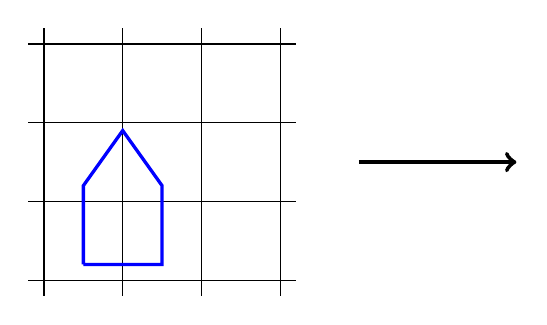
\begin{tikzpicture}
			\foreach \x in {0,1,2,3} {
				\draw (-.2,\x) -- (3.2,\x);
				\draw (\x,-.2) -- (\x,3.2);
			}
			\draw[color=blue,very thick] (.5,.2) -- (1.5,.2) -- (1.5,1.2) -- (1,1.9) -- (.5,1.2) -- (.5,.2);
			
			\draw [ultra thick,->] (4,1.5) -- (6,1.5);
		\end{tikzpicture} \hspace{.3cm}
		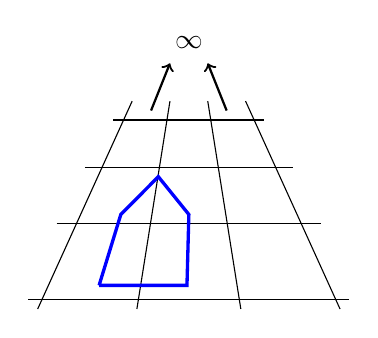
\begin{tikzpicture}[scale=1.2]
			\draw (-.2,0) -- (3.2,0);
			\draw (.1,.8) -- (2.9,.8);
			\draw (.4,1.4) -- (2.6,1.4);
			\draw (.7,1.9) -- (2.3,1.9);
			
			\draw (-.1,-.1) -- (.9,2.1);
			\draw (.95,-.1) -- (1.3,2.1);
			\draw (2.05,-.1) -- (1.7,2.1);
			\draw (3.1,-.1) -- (2.1,2.1);
			
			\draw [color=blue, very thick] (.55,.15) -- (.78,.9) -- (1.177,1.3) -- (1.5,.9) -- (1.48,.15) -- (.55,.15);
			\draw [thick,->] (1.1,2.0) -- (1.3,2.5);
			\draw [thick,->] (1.9,2.0) -- (1.7,2.5);
			\draw (1.5,2.55) node[above]{$\infty$};
		\end{tikzpicture}
		\caption{Ergänzung des zweidimensionalen affinen Raums zur projektiven Ebene.}
	\end{figure}
\end{bem}

Zwei Parallelen $g(a,1,c)$ und $g(a,1,d)$ sollen sich dann schneiden, auch rechnerisch. Wir lösen das so, dass in unserer neuen "Ebene" eine dritte "Koordinate" $z$ hinzukommt, welche bei diesen Parallelen also $=0$ sein müsste, wie folgt:

\begin{defn}[projektive Ebene]
	Die \Index{projektive Ebene} über $k$ ist die Menge
	\[ \PP^2(k) = \{ [y_1 : y_2 : y_3] : y_i \in k \text{ nicht alle } 0\}\]
	mit der Vereinbarung, dass $[y_1 : y_2 : y_3] = [z_1 : z_2 : z_3]$ genau dann gilt, wenn es ein $\lambda \in k \setminus \setnull$ gibt mit $y_1 = \lambda z_1, y_2 = \lambda z_2$ und $y_3 = \lambda z_3$.
\end{defn}

\begin{defn}[projektive Ebene (formal)]
	$\PP^2(k)$ ist die Menge der Äquivalenzklassen in $k^3$ bezüglich der Äquivalenzrelation
	\[ (y_1,y_2,y_3) \sim (z_1,z_2,z_3) \quad :\Leftrightarrow \quad \exists \lambda \in k \setminus \setnull : y_i = \lambda z_i, i = 1, 2, 3 \]
	das heißt $\PP^2(k) := (k^3 \setminus \{(0,0,0)\} / \sim$. \\
	Wir schreiben $[y_1 : y_2 : y_3]$ für die Äquivalenzklasse, die von $(y_1,y_2,y_3)$ repräsentiert wird und nennen sie einen \bet{projektiven Punkt}. $y_1,y_2,y_3$ nennen wir \bet{projektive Koordinaten} von $[y_1: y_2 : y_3]$.
\end{defn}

\begin{bem}
	Ist $y_3 \neq 0$, gilt $[y_1 : y_2 : y_3] = \benbrace*{\frac{y_1}{y_3} : \frac{y_2}{y_3} : 1}$, das heißt die dritte (oder jede andere Koordinate $\neq 0$) kann dann auf $1$ gebracht ("normiert") werden.
\end{bem}

Einem projektiven Punkt $[x:y:z]$ entspricht in unserem Modell in $k^3$ die Ursprungsgerade $\{(\lambda x, \lambda y, \lambda z) : \lambda \in k\}$. Diese Punkte sind entweder $[x:y:1]$ oder $[x:y:0]$ mit $x,y \in k$ (nicht $[0:0:0]$!). \\
Zum Beispiel durch die Abbildung
\begin{equation}
\begin{aligned}
	\iota\colon \aff^2(k) &\longrightarrow \PP^2(k) \\
	(x,y) &\longmapsto [x:y:1]
\end{aligned}
\end{equation}
kann die affine Ebene in die projektive eingebettet werden (d.h. $\iota$ ist injektiv).
\begin{figure}[h]
	\centering
	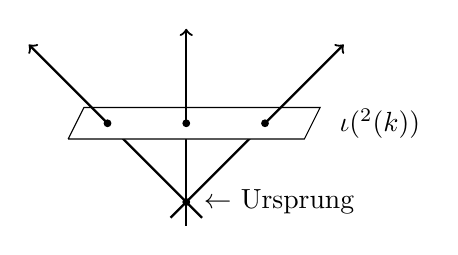
\begin{tikzpicture}
		\draw [thick] (.2,-.2) -- (-1,1);
		\draw [thick] (0,-.3) -- (0,1);
		\draw [thick] (-.2,-.2) -- (1,1);
		
		\draw [fill=white] (-1.5,.8) -- (1.5,.8) -- (1.7,1.2) -- (-1.3,1.2) -- (-1.5,.8);
		
		\draw (-1,1) node[fill,circle,inner sep=1pt]{};
		\draw (0,1) node[fill,circle,inner sep=1pt]{};
		\draw (1,1) node[fill,circle,inner sep=1pt]{};
		\draw (0,0) node[fill,circle,inner sep=1pt]{};
		
		\draw [thick, ->] (-1,1) -- (-2,2);
		\draw [thick, ->] (0,1) -- (0,2.2);
		\draw [thick, ->] (1,1) -- (2,2);
		
		\draw (1.7,1) node[align=left,label={right:$\iota(\aff^2(k))$}] {};
		\draw (.1,0) node[right,align=left] {$\leftarrow$ Ursprung};
	\end{tikzpicture}
\end{figure}

\begin{bem}
	Aber $\PP^2(k)$ enthält zusätzlich noch die projektiven Punkte $[x:y:0]$ mit $x,y \in k$ (nicht $x=y=0$). Offenbar ist $\{[x:y:0] : x,y \in k, \text{ nicht } x = y = 0\}$ eine Gerade in $\PP^2(k)$, die wir \Index{unendlich ferne Gerade} $g_\infty$ nennen möchten, denn mit $j \colon k \rightarrow g_\infty, x \mapsto [x:1:0]$ lässt sich $k$ darin einbetten (das heißt $j$ ist injektiv), wobei auffällt, dass $g_\infty \setminus \im(j)$ aus genau den weiteren Punkt $\oh := [1:0:0]$ besteht, das heißt $g_\infty \setminus \im(j) = \{\oh\}$.
\end{bem}

\begin{bem}
	Somit: $\PP^2(k) = \iota(\aff^2(k)) \sqcup \underbrace{\textcolor{green}{j(k)} \sqcup \textcolor{red}{\{\oh\}}}_{=g_\infty}$ \marginnote{disjunkte Vereinigung}
\begin{figure}[h]
\centering
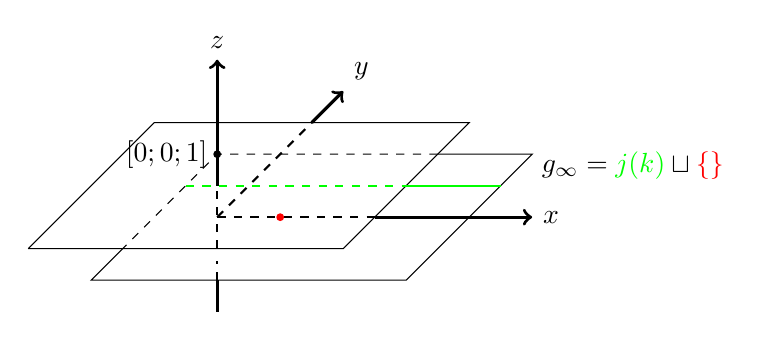
\begin{tikzpicture}[scale=0.8]
	\draw (-1.5,-.5) -- (-2,-1) -- (3,-1) -- (5,1) -- (3.5,1);
	\draw [dashed] (3.5,1) -- (0,1) -- (-1.5,-.5);
	\draw (-3,-.5) -- (2,-.5) -- (4,1.5) -- (-1,1.5) -- (-3,-.5);
	
	
	\draw [very thick] (0,-1.5) -- (0,-1);
	\draw [thick, dashed] (0,-1) -- (0,-.7);
	\draw [thick, dashed] (0,-.5) -- (0,.5);
	\draw [very thick, ->] (0,0.5) -- (0,2.5) node[above] {$z$};
	\draw [thick, dashed] (0,0) -- (2.5,0);
	\draw [very thick, ->] (2.5,0) -- (5,0) node[right] {$x$};
	\draw [thick, dashed] (0,0) -- (1.5,1.5);
	\draw [very thick, ->] (1.5,1.5) -- (2,2) node[anchor=south west] {$y$};
	
	\draw [color=green, thick, dashed] (-.5,.5) -- (3,.5);
	\draw [color=green, thick] (3,.5) -- (4.5,.5);
	
	\draw (1,0) node[fill,circle,inner sep=1pt,color=red]{};
	\draw (1,0) node[color=red,anchor=south west]{$\oh$};
	
	\draw (0,1) node[fill,circle,inner sep=1pt]{};
	\draw (0,1) node [left,align=right] {$[0;0;1]$};
	
	\draw (5,1.2) node[anchor=north west,align=left] {$g_\infty = \textcolor{green}{j(k)} \sqcup \textcolor{red}{\{\oh\}}$};
\end{tikzpicture}
\hspace{1.5cm}
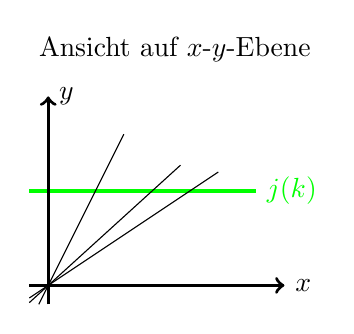
\begin{tikzpicture}[scale=1.2]
	\draw [very thick, color=green] (-.2,1) -- (2.2,1) node[right]{$j(k)$};
	\draw [very thick,->] (-.2,0) -- (2.5,0) node [right] {$x$};
	\draw [very thick,->] (0,-.2) -- (0,2) node [right] {$y$};
	
	\draw (-.1,-.2) -- (.8,1.6);
	\draw (-.2,-.1818) -- (1.4,1.2727);
	\draw (-.2,-.1333) -- (1.8,1.2);
	
	\draw (-.2,2.5) node[right,align=left]{Ansicht auf $x$-$y$-Ebene};
\end{tikzpicture}	
\end{figure}
\end{bem}

Die in $\aff^2(k)$ parallelen Geraden $g(a,1,c) = \{(x,y) \in k^2 : ax + y + c = 0\} = \{(x,-ax-c) : x \in k\}$ und $g(a,1,d)$ müssen die projektiven Punkte $[x:-ax-c:1]$ und $[x:-ax-d:1]$ enthalten. \\
Das klappt, wenn die Gleichung $ax + y \{c,d\} = 0$ zu $ax + y + \{c,d\}z = 0$ ergänzt wird. Sie schneiden sich dann im unendlich fernen Punkt $[1 : -a : 0] = \benbrace*{-\frac{1}{a} : 1 : 0}$, welcher die gemeinsame Steigung $-a$ angibt bzw. die gemeinsame "Richtung" $(1,-a)$. Die gemeinsame Richtung $(1,-a)$ wird zum gemeinsamen Schnittpunkt $\benbrace*{-\frac{1}{a} : 1 : 0}$ erklärt.

\begin{defn}[projektive Gerade]
	Eine \Index{projektive Gerade} ist eine Teilmenge von $\PP^2(k)$ der Form
	\[ g(a,b,c) = \{ [x:y:z] : ax+by+cz = 0\} \text{ für } (a,b,c) \in k^3 \setminus \setnull \]
	Man sagt, die "projektive" Gleichung $ax+by+cz = 0$ ist "durch Homogenisierung" aus $ax+by+c = 0$ entstanden: Durch die Ergänzung mit $z$ haben nun alle Summanden $ax,by,cz$ denselben Grad $1$ als Polynom aus $k[x,y,z]$. Dieses Prinzip werden wir für allgemeinere Kurven für den Übergang vom Affinen ins Projektive übernehmen. Projektive Geraden werden uns in der Form von Tangenten dann wiederbegegnen.
\end{defn}

\minisec{Beispiel und Bemerkung}
	Die projektiven Geraden $g(a,1,c),g(a,1,d)$ schneiden sich in $\penbrace*{-\frac{1}{a}:1:0} \in g_\infty$. Durch je zwei verschiedene Punkte des $\PP^2(k)$ führt genau eine projektive Gerade.
	
\subsubsection{Affine Kurven}
\label{subsub:2.2.2}
	Doch zunächst möchten wir im affinen Raum allgemeinere Kurven untersuchen. Dazu benutzen wir Polynome zu ihrer Beschreibung.
	
\begin{defn}[affine Kurve]
	Sei $f \in k[x,y]$ ein Polynom über $k$ in zwei Variablen $x$ und $y$. Wir bezeichnen die Menge der Nullstellen von $f$ in $k \times k = \aff^2(k)$ als
	\[ \cc_f(k) := \{(u,v) \in \aff^2(k) : f(u,v) = 0\}\]
	Jede solche Nullstellenmenge $\cc_f(k)$ nennen wir eine \Index{affine Kurve}. Ist klar, welches Polynom $f$ vorliegt, schreiben wir auch kurz $\cc(k)$ für $\cc_f(k)$. Geraden sind spezielle affine Kurven (zu linearen Polynomen $f(x,y,z) = ax+by+c$).
\end{defn}

\begin{bem}
	Für uns ist interessant, Kurven über verschiedenen Körpern $k$ zu studieren. Der Fall eines endlichen Körpers ist für Anwendungen interessant, weil dann alle Kurven aus nur endlich vielen Punkten bestehen können.
\end{bem}

\begin{bsp}
	Sei $k = \RR$ und $f(x,y) = y-x^3-x$. Die Nullstellenmenge $\cc_f(k)$ besteht dann aus allen Punkten $(x,y) \in k^2$, welche die Gleichung $y = x^3 + x$ erfüllen. Das reelle Schaubild sieht so aus:
	\begin{figure}[h]
	\centering
	\begin{tikzpicture}[scale=.7]
		\draw [->] (-3,0) -- (3,0) node[above] {$x$};
		\draw [->] (0,-3) -- (0,3) node[right] {$y$};
		\draw [domain=-1.2:1.2,smooth,variable=\x,blue] plot ({\x},{\x*\x*\x + \x});
	\end{tikzpicture}
	\caption{Die Menge $\{(x,y) \in \RR^2 : y = x^3 + x\}$.}
	\end{figure}
	Für $k = \FF_5$ können nur wenige Punkte auf der "Kurve" liegen: Die Tabelle
	\begin{center}
	\begin{tabular}{c|c|c|c|c|c}
	$a$ & $0$ & $1$ & $2$ & $3$ & $4$ \\ 
	\hline $a^3$ & $0$ & $1$ & $3$ & $-3$ & $-1$ \\ 
	\hline $a^3+a$ & $0$ & $2$ & $0$ & 0 & $3$
	\end{tabular} 
	\end{center}
	zeigt, dass $\cc_f(\FF_5) = \{ (0,0), (1,2), (2,0), (3,0), (4,3)\}$ ist, und mit $f_0(x,y) = y^2 - x^3 - x$ haben wir $\cc_{f_0}(\FF_5) = \{(0,0),(2,0),(3,0)\}$. \\
	Ist $\tilde{k} \subseteq k$ ein Teilkörper von $k$ (wie zum Beispiell $\QQ \subseteq \RR$), so folgt auch stets $\cc_f(\tilde{k}) \subseteq \cc_f(k)$. Unsere Kurvenpunkte in $\aff(\FF_5)$ finden wir deswegen zum Beispiel in $\aff(\FF_{25})$ wieder.
\end{bsp}

\begin{defn}[Tangente]
	Eine (affine) \Index{Tangente} an eine affine Kurve $\cc_f(k)$ im Punkt $(a,b) \in \cc_f(k)$ ist die Gerade
	\[ t_f(a,b) = \{ (u,v) : \frac{\der f}{\der x} (a,b)x + \frac{\der f}{\der y}(a,b)y + d = 0\},\]
	falls diese existiert (wir brauchen, dass $\frac{\der f}{\der x}(a,b), \frac{\der f}{\der y}(a,b)$ nicht beide $=0$). Dabei ist $d \in k$ so gewählt, dass $(a,b) \in t_f(a,b)$ gilt.
\end{defn}

\begin{bem}
	Es ist nicht klar, ob Tangenten stets eindeutig existieren. Affine Kurven können sich selbst schneiden oder scharfe "Spitzen" haben. Siehe z.B. Abbildung~\ref{fig:bsp} in Abschnitt~\ref{sec:para0}.
\end{bem}

\begin{defn}[singulärer Punkt]
	Die affine Kurve $\cc_f(k)$ heißt \bet{singulär im Punkt} $(a,b) \in \cc_f(k)$, falls $\frac{\der f}{\der x}(a,b) = \frac{\der f}{\der y}(a,b) = 0$ gilt. \index{singulär}
\end{defn}

\begin{bem}
	Affine Kurven, die in keinem Punkt singulär sind, haben überall eine wohldefinierte Tangente.
\end{bem}

\begin{bem}
	Es kann vorkommen, dass $\cc_f(k)$ gar keine singulären Punkte enthält, wohl aber über einem Erweiterungskörper von $k$, wie etwa $\overline{k}$, dem algebraischen Abschluss über $k$.
\end{bem}

\begin{bsp}
	Für $f(x,y) = y^2 - x^4 - 2x^2 - 1$ hat $\cc_f(\RR)$ keine singulären Punkte: Es ist $\frac{\der f}{\der x}(a,b) = -4a^3 - 4a = -4a(a^2+1), \frac{\der f}{\der y}(a,b) = 2b$. Allerdings sind $(i,0),(-i,0) \in \CC$ singuläre Punkte in $\cc_f(\CC)$, wo $\CC = \overline{\RR}$.
\end{bsp}

\begin{bsp}
	Sei $f(x,y) = y^2 - x^3 - x$ und $k = \FF_p$. Die Ableitungen sind $\frac{\der f}{\der x} (x,y) = -3x^2-1, \frac{\der f}{\der y}(x,y) = 2y$, das heißt die singulären Punkte $(a,b)$ sind die mit $b^2 = a^3 + a$, $-3a^2 = 1, 2b=0$.\begin{itemize}
		\item Für $p \neq 2$ ist $2b = 0$ nur für $b = 0$ richtig, dann ist $0 = a(a^2+1)$ und $3a^2 = -1$. Es folgt $0 = a(3a^2 + 3) = 2a$ und wegen $p \neq 2$ folgt $a = 0$ im Widerspruch zu $3^2=-1$. Also existieren keine singulären Punkte für $p \neq 2$.
		\item Für $p = 2$ ist $\cc_f(\FF_2) = \{(0,0),(1,0)\}$. Es ist $\frac{\der f}{\der x} (1,0) = 0 = \frac{\der f}{\der y}(1,0)$, das heißt $(1,0)$ ist singulärer Punkt.
	\end{itemize}
\end{bsp}